
%%%%%%%%%%%%%%%%%%%%%%% file typeinst.tex %%%%%%%%%%%%%%%%%%%%%%%%%
%
% This is the LaTeX source for the instructions to authors using
% the LaTeX document class 'llncs.cls' for contributions to
% the Lecture Notes in Computer Sciences series.
% http://www.springer.com/lncs       Springer Heidelberg 2006/05/04
%
% It may be used as a template for your own input - copy it
% to a new file with a new name and use it as the basis
% for your article.
%
% NB: the document class 'llncs' has its own and detailed documentation, see
% ftp://ftp.springer.de/data/pubftp/pub/tex/latex/llncs/latex2e/llncsdoc.pdf
%
%%%%%%%%%%%%%%%%%%%%%%%%%%%%%%%%%%%%%%%%%%%%%%%%%%%%%%%%%%%%%%%%%%%


\documentclass[runningheads,a4paper]{llncs}

\usepackage{amssymb}
\setcounter{tocdepth}{3}
\usepackage{graphicx}

\usepackage{alltt}

%%%%%%%%%%%%%%%%%
\usepackage{listings}
\lstset{
  basicstyle=\ttfamily,
  mathescape
}
%%%%%%%%%%%%%%%%%
% table
\usepackage{multirow}
\usepackage[table,xcdraw]{xcolor}

\usepackage[T1]{fontenc}
\usepackage[utf8]{inputenc}
\usepackage{tabularx,ragged2e,booktabs,caption}
\newcolumntype{C}[1]{>{\Centering}m{#1}}
\renewcommand\tabularxcolumn[1]{C{#1}}
%%%%%%%%%%%%%%%%%%

\usepackage{url}
\urldef{\mailsa}\path|{jhyun19, wsnah}@skku.edu| 
\urldef{\mailsb}\path|{xuyan}@ntu.edu.sg|   
\newcommand{\keywords}[1]{\par\addvspace\baselineskip
\noindent\keywordname\enspace\ignorespaces#1}

\begin{document}

\mainmatter  % start of an individual contribution

% first the title is needed
\title{Short-Term Load Forecasting of Australian National Electricity Market by Hierarchical Extreme Learning Machine}

% a short form should be given in case it is too long for the running head
\titlerunning{STLF of Australian NEM by Hierarchical ELM}

% the name(s) of the author(s) follow(s) next
%
% NB: Chinese authors should write their first names(s) in front of
% their surnames. This ensures that the names appear correctly in
% the running heads and the author index.
%
\author{Park Jee Hyun%
%\thanks{Please note that the LNCS Editorial assumes that all authors have used
%the western naming convention, with given names preceding surnames. This determines
%the structure of the names in the running heads and the author index.}%
\and Xu Yan\and Nah Wan Soo}
%
\authorrunning{STLF of Australian NEM by Hierarchical ELM}
% (feature abused for this document to repeat the title also on left hand pages)

% the affiliations are given next; don't give your e-mail address
% unless you accept that it will be published
\institute{SungKyunKwan University, Electronic and Electrical Engineering,\\
2066, Seobu-ro, Jangan-gu, Suwon-si, Gyeonggi-do, Republic of Korea\\
\mailsa\\
\mailsb\\
\url{http://www.skku.ac.kr/}}

%
% NB: a more complex sample for affiliations and the mapping to the
% corresponding authors can be found in the file "llncs.dem"
% (search for the string "\mainmatter" where a contribution starts).
% "llncs.dem" accompanies the document class "llncs.cls".
%

\toctitle{STLF of Australian NEM by Hierarchical ELM}
\tocauthor{Authors' Instructions}
\maketitle


\begin{abstract}
Artificial Neural Network(ANN) is an effective approach for short-term load forecasting (STLF). While accurate load forecasting is pivotal for the economic and secure operation of the power system, there have been continuous efforts to achieve high load forecasting accuracy. There are two main ways to do this: the first is the improvement of the performance of the learning algorithm, and the second is how well the data features are extracted through the pre-processing process. In this paper, we design Hierarchical-Extreme Learning Machine (H-ELM) based STLF model for forecasting the electricity load of Australian National Electricity Market (NEM) data. Owing to the very fast training/tuning speed of feed-forward neural network and multilayer concept, the H-ELM model, like the Extreme Learning Machine (ELM), is able to make fast and efficient predictions, while overcoming the instability of the forecast, which was a drawback of ELM. In addition, the H-ELM model shows better performance due to data pre-processing.
\keywords{Hierarchical-extreme learning machine (H-ELM), Extreme learning machine (ELM), Data pre-processing, Short-term load forecasting (STLF)}
\end{abstract}


\section{Introduction}

Predicting future demand load for electricity is considered an essential process in power system operation. With the development towards smart grids, the forecasting results of higher accuracy are required \cite{importance_load_forecast}. Short term load forecasting (STLF) is a prediction of the load ahead of an hour to a few days. The STLF has a significant impact on the generation scheduling and reserving activities of the power system \cite{ensemble_elm}. In other words, good quality STLF is very important for economical aspect and contributes to reliability of power system \cite{reliability}, \cite{economic}. Therefore, it is very important to develop an STLF model with higher performance.

Over the past few years, much research has been done on the Extreme Learning Machine (ELM), and ELM has been applied to a number of areas, including STLF, resulting in remarkable results. ELM is faster and more efficient than traditional Artificial Neural Network (ANN), and shows better generalization performance \cite{elm_theory}. In addition, there are advantages to avoid problems such as stopping criteria, learning rate, learning epochs and local minima that existing ANNs often encounter \cite{elm_better_than_ann}. However, there is a disadvantage in that the results of forecasting are unstable due to the random generation of input parameters during ELM training \cite{ensemble_elm}.

Recently, a novel learning technology called Hierarchical-Extreme Learning Machine (H-ELM) was proposed \cite{helm}. H-ELM is a multi-layered ELM-based artificial intelligence network. It consists of multi-layer forward encoding part extracting high-level sparse features from input data for training and original ELM part performing final decision. According to previous studies \cite{helm}, H-ELM has better performance than ELM. And, if data pre-processing is used in the field of predicting time series data, more accurate forecasting results will be obtained even if the same data is used \cite{pre_process}. In this paper, experiments were conducted to confirm the prediction performance improvement by inputting data through appropriate data preprocessing to the STLF model using H-ELM instead of ELM.

The remainder of the paper is organized as follows. Section 2 introduces the ELM theory and H-ELM framework; Section 3 introduces the data used in the experiment in this paper; In Section 4, we introduce the experimental design to evaluate the performance according to the type of STLF model and data preprocessing; The results for the experiment are given in Section 5, and in Section 6 the conclusion drawn through the experimental results is described.


\section{Hierarchical Extreme Learning Machine}

\subsection{ELM theory}

The ELM is a learning technology working for generalized single hidden layer feedforward networks (SLFN) and it consists of three layers \cite{elm_theory}: input layer, hidden layer and output layer as shown in Figure 1.

\begin{figure}
\centering
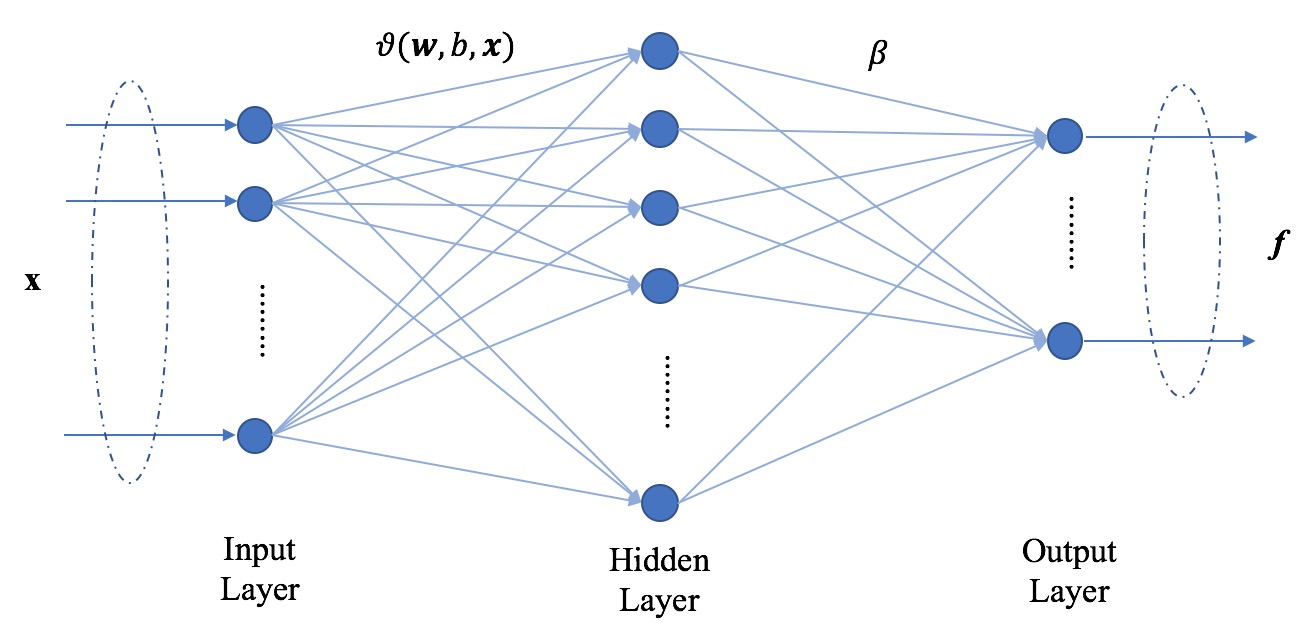
\includegraphics[width=9.6cm]{elm_figure}
\caption{Structure of a SLFN}
\label{fig:elm_figure}
\end{figure}

Given a training data set with $N$ samples, the output function of the SLFN with $L$ hidden nodes and activation function $\vartheta$. The activation function is expressed as following

\begin{equation}
f_{L}(x_{j})=\sum_{L}^{i=1}\beta _{i}\vartheta (\omega _{i}x_{j}+b_{i}) = t_{j}, j=1, 2, ..., N
\end{equation}


ELM is completely different from traditional iterative learning algorithms as it randomly selects the input weights and biases for hidden nodes,  $\omega$ and $b$ and analytically calculates the output weights, $\beta$, by finding least-square solution \cite{neuro1}. According to ELM theory \cite{neuro1}, (1) can be rewritten into a compact format as follows

\begin{equation}
\textbf{H}\beta =\mathbf{T}
\end{equation}

For a training data set, given the activation function and hidden node number, the ELM learning can be summarized as the following major three steps:

\begin{lstlisting}
Step 1. Randomly generate the input weights $\omega _{i}$ and $b_{i}$,
        $1\leq i\leq N$;
Step 2. Calculate the hidden layer output matrix $\mathbf{H}$; and 
Step 3. Calculate output weights matrix $\beta =\mathbf{H^{\dagger }T}$;
   
where $\mathbf{H^{\dagger}}$ is the Moor–Penrose (MP) generalized inverse 
of $\mathbf{H}$ $\cite{neuro1}$.
\end{lstlisting}

Unlike the other traditional ANN learning algorithms, ELM requires no iteratively adjustments of network parameters during the training. In other words, once ELM parameters of hidden layers of the ELM are generated randomly, it does not need to be tuned. Therefore, its training speed can be thousands of times faster \cite{elm_better_than_ann}. And, as proved in \cite{neuro1}, it can not only reach the minimized training error $\left \| \mathbf{H}\beta -\mathbf{T} \right \|$, but also the smallest norm of output weights $\left \| \beta \right \|$. It is known that the feed-forward neural network achieves good generalize performance as the training error and the norm of weight become smaller \cite{neuro2}. Further, ELM can avoid difficulties such as stopping criteria, learning rate, learning epochs and local minima that can be commonly encountered by traditional algorithms.

Due to the characteristics of the ELM based SLFN, we can obtain very short training time, excellent efficiency and good generalize performance \cite{elm_better_than_ann}. However, it randomly selects the input weights and biases for hidden nodes, and cause a crux in the stability of its outputs \cite{ensemble_elm}. 

\subsection{H-ELM framework}

Over the past several years, ELM has been developed and applied to various fields. Due to the unique characteristics of ELM, we were able to gain many advantages such as extremely fast training, good generalization, and universal approximation/ classification capability. However, it is considered that the instability of output is a disadvantage, and it is known that only one hidden layer cannot perform learning of high-level features of input data. These issues are expected to be solved by the H-ELM, which is a feed-forward neural network with multiple-layers concept, and it will be confirmed through the experiments designed in this paper.

According to \cite{helm}, unlike the traditional gradient-based framework, the HELM consists of two parts as shown in Figure 2: 1) unsupervised hierarchical feature representation and 2) supervised feature classification. For first part, ELM-based autoencoder is built in to extract multilayer sparse features of the input data. For second part, the original ELM-based regression is placed to conduct final decision making. In 1) unsupervised feature learning phase, which is the first phase of H-ELM structure, it receives raw input data and projects it to the ELM random feature space, which plays an important role in extracting hidden feature information of input training data. Eventually, high-level sparse features can be obtained as output values through N-layer unsupervised learning, which is then passed to the input data of the second stage 2) supervised feature classification. In this step, the final decision is made through regression, which is the same process as the existing ELM. Since H-ELM receives input of high-level sparse features obtained from unsupervised feature learning, instead of raw input data, it is able to obtain more accurate and stable performance.

The experiments designed in the back will confirm that H-ELM shows better performance than ELM.

\begin{figure}
\centering
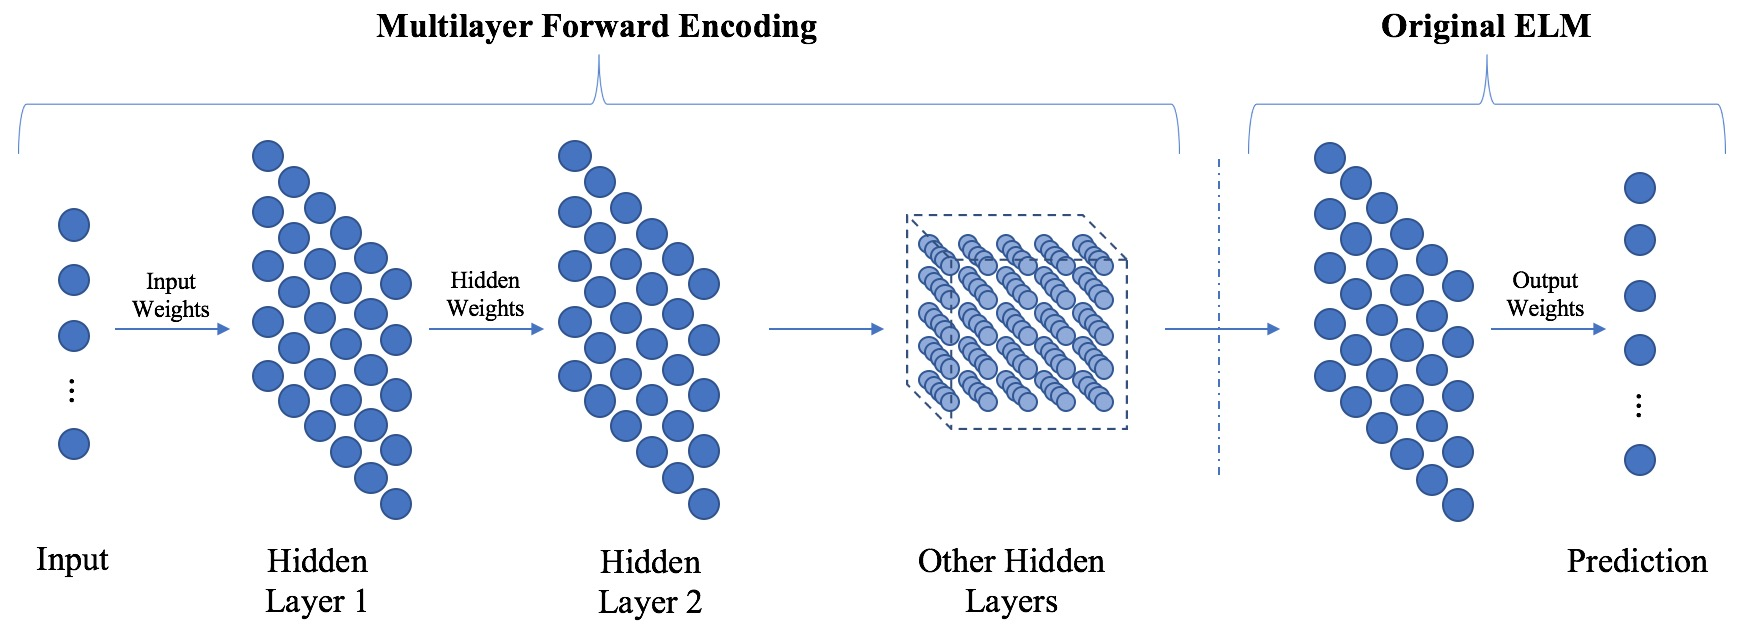
\includegraphics[width=12.1cm]{helm_figure}
\caption{Overall framework of H-ELM, which is divided into two phases:
multilayer forward encoding followed by the original ELM-based regression}
\label{fig:helm_figure}
\end{figure}

\section{Data used in experiments}

\subsection{Australian NEM}

The NEM metrology procedure define a requirement for calculation of a Net System Load profiles (NSLP) for Victoria, New South Wales (NSW), Australian Capital Territory (ACT), South Australia (SA), Queensland (QLD) and Tasmania (TAS) and a Controlled Load profiles (CLP) for each network area in NSW and SA and two CLP for the Energex, which is an Australian electric power distribution company owned by the Government of Queensland, distribution area \cite{url_nem}. Both types of profiles have data recorded every 30 minutes (48 points per day). 

In this paper, we focused on NSLP and load profile of NSW region from 1 January 2006 to 31 December 2015 is used. The value corresponding to the $ k $-th date of the data will be expressed in the expression (3).

\begin{equation}
\left [ P_{k}(1), P_{k}(2), ..., P_{k}(48) \right ]
\end{equation}


\subsection{Australian Bureau of Meteorology}

Previous studies have shown a strong correlation between future load and weather variables \cite{weather1}, \cite{weather2}. Based on this fact, this paper will use Australian Government Bureau of Meteorology (BOM) weather data with NEM data. The Australian Government Bureau of Meteorology is the national meteorological authority for Australia. It provides weather forecasts, warnings and observations for all states and territories of Australia. There is also information about climate, hydrology and other weather services such as weather charts, radar images, satellite images and marine weather \cite{url_bom}. 

In this paper, we choose to use the maximum temperature, minimum temperature, rainfall, and solar exposer data by date (4 points per day) among the weather data provided in the BOM. The data used are for NSW region from 1 January 2006 to 31 December 2015. The value corresponding to the $ k $-th date of the data will be expressed in the espression (4).

\begin{equation}
\left [ T_{k}^{Max}, T_{k}^{min},  R_{k}, S_{k}\right ]
\end{equation}

\section{Implementation structure}

\subsection{Data pre-processing strategies}

Data pre-processing is an important process for better forecsting performance \cite{preprocessing} and is a process for determining how to configure the feature input dataset. Sufficient and well-defined feature input dataset is required to obtain valid predictions in the forecasting experiment \cite{welldefine_feature}. If the weather data from the BOM to be used in this paper were time series data at 30-minute intervals with 48 points recorded per day, this data could be used directly as feature input dataset and NEM load data could be used as label input data. However, all the weather data that can be obtained from the BOM is time series data, only one value is recorded per day. Using these data directly as feature input dataset can not provide sufficient features to train the STLF model and will result in inaccurate and invalid forecasting results.

To overcome this problem, we will use data pre-processing to include the historical load data from the NEM in the feature input dataset consisting of the weather data of the BOM. Which historical load data to  be included in the feature input dataset will be described in the following correlation study. This is a strategy to include historical load data in the feature input dataset component because it can not provide sufficient features to construct the feature input dataset with only weather data for the STLF model training. In short, the forecasting method is based on historical load data and takes weather forecast as a hint to predict future load data. It will be confirmed from the following experiment that the prediction obtained through data pre-processing which intentionally increases the feature input dataset in this way can allow more accurate and valid results.

\subsection{Correlation study}

In this paper, we use the correlation between data given as a measure to select the most suitable input data for model training, and the correlation analysis based on Pearson’s correlation coefficient (PCC). Pearson's correlation coefficient is the covariance of the two variables, which will be the electricity load variables of each half an hour in our studies, divided by the product of their standard deviations, which can be calculated as follows

\begin{equation}
\rho _{X, Y}=\frac{\sum_{n}^{i=1} (X_{i}-\bar{X})(Y_{i}-\bar{Y})}{\sqrt{\sum_{n}^{i=1} (X_{i}-\bar{X})^{2}}\sqrt{\sum_{n}^{i=1} (Y_{i}-\bar{Y})^{2}}}
\end{equation}

We have already stated that NEM load data will be used not only as label data but also as feature data. The question is, which part and how much of load data to use as feature data. Selecting the right amount of data and the appropriate features of data as input data is an important process that must be performed first for accurate load forecasting \cite{feature_select}. Therefore, in this paper, we decided to adopt the method of selecting load data of two dates with the highest pcc value as input feature data. The results of the PCC calculations in Figure 3 confirm that these two dates are the same day of the previous day and the previous week.

\begin{figure}
\centering
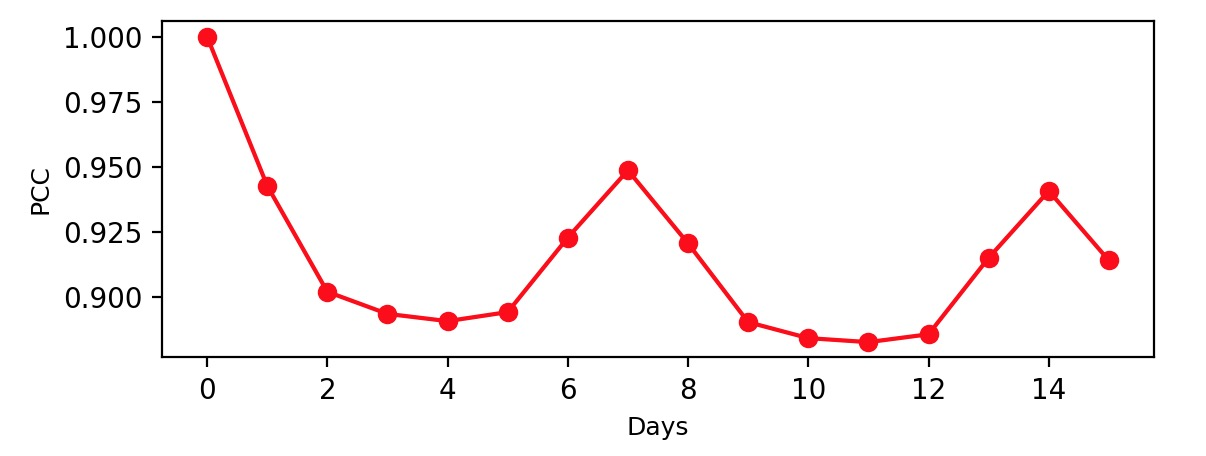
\includegraphics[width=12.1cm]{pcc_figure}
\caption{Pearson's correlation coefficient against days}
\label{fig:helm_figure}
\end{figure}

\subsection{Architecture}

The architecture of the STLF model for NEM is shown in Figure 4. The learning model part described in Fig 3 will consist of ELM or H-ELM. In the following, we will check performance differences between ELM and H-ELM. This architecture is divided into two phases: a) training and b) testing. In the a) training phase, the learning model receives the feature vector obtained through the data pre-processing process and performs model training. The STLF model trained in this phase is used in the next phase. In the b) testing phase, the feature vector is input and forecasting is performed based on the STLF model trained in the previous process. For reference, the input features of the training phase and the testing phase are of different contents extracted from training data and testing data, respectively. 

Performance of accuracy evaluation for forecasting will be performed using mean absolute squared error (MAPE) and mean absolute error (MAE), which are calculated as follows
\begin{equation}
MAPE(\%)=\frac{1}{N} \sum_{N}^{i=1} \frac{\left | P_{k}(i)-\hat{P}_{k}(i) \right |}{\left | P_{k}(i) \right |}\times 100
\end{equation}

\begin{equation}
MAE=\frac{1}{N} \sum_{N}^{i=1} \left | P_{k}(i)-\hat{P}_{k}(i) \right |
\end{equation}
where $P_{k}(i)$ and $\hat{P}_{k}(i)$ are, respectively, the real and forecasted value of electricity load, $N$ is the total number of the points being forecasted. In order to evaluate the predictive stability of the STLF model, we will use standard deviation of each distribution of MAPE and MAE obtained as a result after performing 1,000 repetitive prediction experiments. 

\begin{figure}
\centering
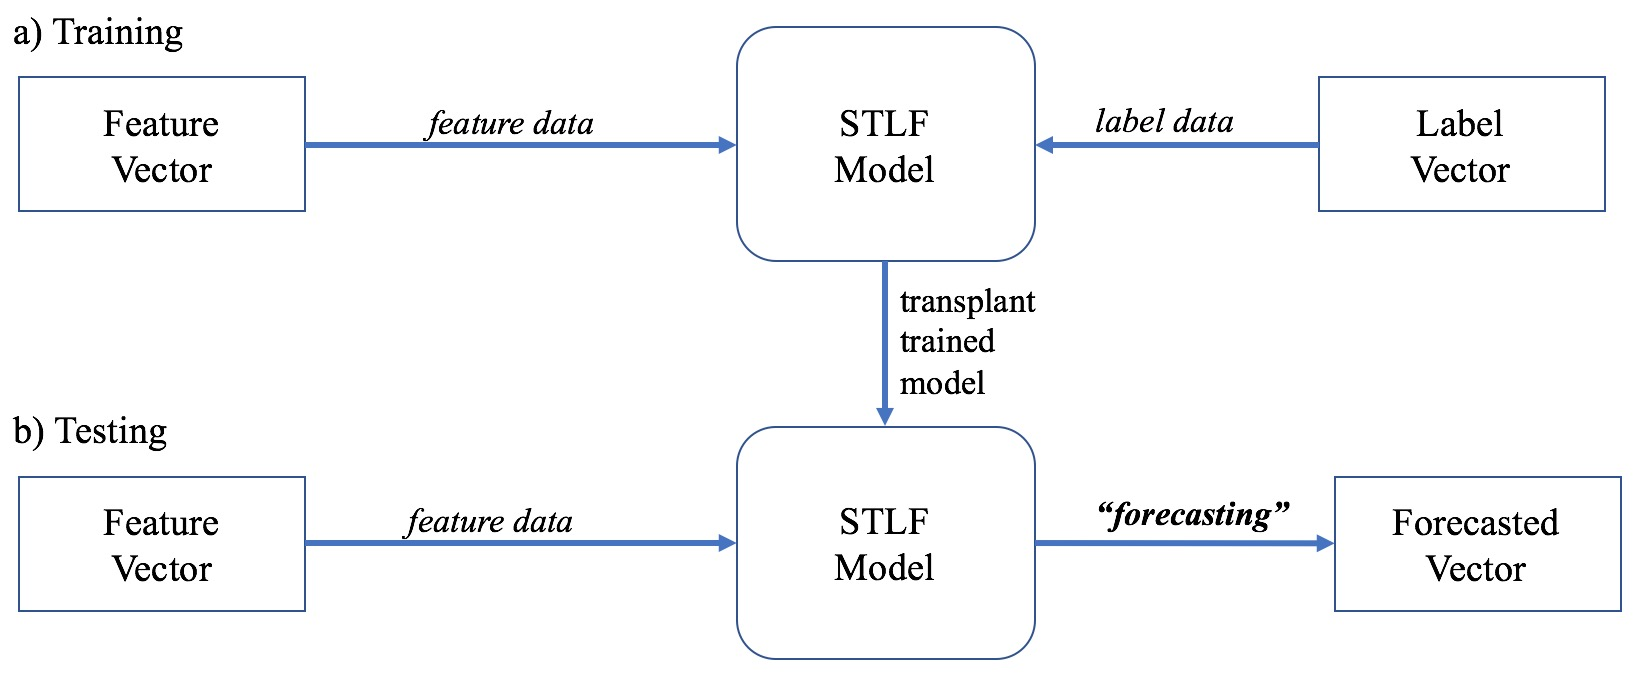
\includegraphics[width=11cm]{structure_figure}
\caption{Architecture of STLF model}
\label{fig:helm_figure}
\end{figure}

\subsection{Input}

To train the STLF model, input data consisting of feature data and label data is required. In this experiment, we will confirm the role of data pre-processing in addition to the performance comparison between ELM and H-ELM. Therefore, we will set up four cases as in Table 1. It should be noted that the all data we use in each case are identical, but will be entered into the each STLF model in different forms through different data pre-processing process. 

In all four cases, the same load data as the $k$-th day will be entered as the label data. In the case 00, which is considered as the most basic data pre-processing process, the weather data of the $k$-th day will be input as feature data. In case 01, the $k$-th day weather data and the $\left ( k-1 \right )$-th day load data corresponding to the previous day's load data will be accompanied. In case 02, the weather data of the $k$-th day and the load data of the $\left ( k-7 \right )$-th day corresponding to the load data of the same day of the week are transmitted as the feature data. Finally, in case 03, the weather data for the $k$-th day and the load data for the $\left ( k-1 \right )$-th day and the $\left ( k-7 \right )$-th day will be input as feature data.

\begin{table}[]
\centering
\renewcommand{\arraystretch}{1.3}
\caption{Cases of input data depending on the data preprocessing}
\label{my-label}
\begin{tabular}{p{19mm} p{49mm} p{49mm}}
\hline
\multicolumn{1}{c}{} & \multicolumn{1}{c}{\textbf{Label data}} & \multicolumn{1}{c}{\textbf{Feature data}}                  \\ \hline
Case 00 & $\left [ P_{k}(1), P_{k}(2), ..., P_{k}(48) \right ]$          & $\left [ T_{k}^{Max}, T_{k}^{min},  R_{k}, S_{k}\right ]$                                                 \\ \hline
Case 01 & $\left [ P_{k}(1), P_{k}(2), ..., P_{k}(48) \right ]$          & \begin{tabular}[c]{@{}l@{}}$\left [ T_{k}^{Max}, T_{k}^{min},  R_{k}, S_{k}\right ]$\\ $\left [ P_{k-1}(1), P_{k-1}(2), ..., P_{k-1}(48) \right ]$\end{tabular}     \\ \hline
Case 02 & $\left [ P_{k}(1), P_{k}(2), ..., P_{k}(48) \right ]$          & \begin{tabular}[c]{@{}l@{}}$\left [ T_{k}^{Max}, T_{k}^{min},  R_{k}, S_{k}\right ]$\\ $\left [ P_{k-7}(1), P_{k-7}(2), ..., P_{k-7}(48) \right ]$\end{tabular}     \\ \hline
Case 03 & $\left [ P_{k}(1), P_{k}(2), ..., P_{k}(48) \right ]$          & \begin{tabular}[c]{@{}l@{}}$\left [ T_{k}^{Max}, T_{k}^{min},  R_{k}, S_{k}\right ]$\\ $\left [ P_{k-1}(1), P_{k-1}(2), ..., P_{k-1}(48) \right ]$\\ $\left [ P_{k-7}(1), P_{k-7}(2), ..., P_{k-7}(48) \right ]$\end{tabular} \\ \hline
\end{tabular}
\end{table}

\subsection{Output}

The designed STLF models output the values according to the multi-output regression method. This output value is the daily load profile, namely the 48 load points corresponding to each half-hour of a day.

\section{Test results}

In this experiment, NEM and BOM data from 2006 to 2015 were used. The data were divided into training data and testing data at a ratio of $8:2$. All the simulations are conducted in MATLAB R2017a platform running on an ordinary PC with 2.4 GHZ CPU. 

\subsection{Optimal number of hidden nodes}

The STLF model designed in this experiment needs to be optimized for maximum performance, which is the task of determining the number of hidden nodes. As the number of hidden nodes is gradually increased, the trend of prediction results using the STLF model is observed, and the number of hidden nodes with the highest accuracy is found and used in the following experiments. For reference, the MAPE method was used to measure accuracy, and the forecasting accuracy result obtained from this optimization process corresponds to the average value of the same 20 repetitive prediction experiments. 

In each case, the number of hidden nodes for the optimization of the STLF model slightly differed, and the results of the experiment for the optimization are shown in Figure 5.

\begin{figure}
\centering
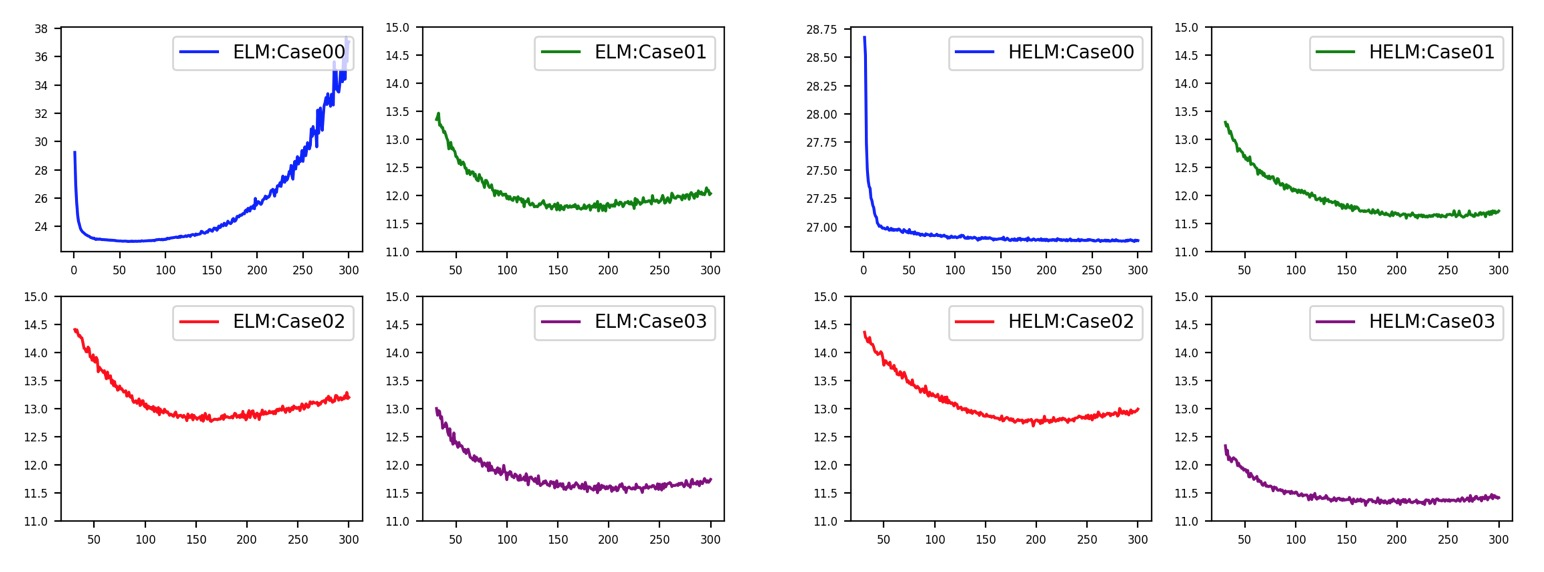
\includegraphics[width=12.3cm]{optimal_figure}
\caption{Hidden node number of ELM and H-ELM against MAPE(\%)}
\label{fig:helm_figure}
\end{figure}

\subsection{Performance comparison between ELM and H-ELM}

The performance of the STLF model designed using ELM and H-ELM is evaluated by two parts. First, the accuracy of the prediction is evaluated using MAPE and MAE. Second, the stability of the prediction is evaluated as the standard deviation of the distribution of the prediction accuracy. In order to measure these two evaluation items, 1,000 identical repeating experiments were conducted for each STLF model. In order to evaluate the accuracy, the mean value of MAPE and MAE values was taken as the final value, and the standard deviation was calculated to evaluate the stability. For each STLF cases, the trains and tests are conducted with the same training and testing datasets. 

Experimental results show that the STLF model devised by H-ELM has smaller standard deviations than MAPE and MAE, which are designed by ELM. And we can confirm that data pre-processing contributes greatly to obtaining small values of both MAPE and MAE. The results are listed in Table 2 and Table 3.

\begin{table}[]
\centering
\renewcommand{\arraystretch}{1.3}
\captionof{table}{Forecasting MAPE and stability} \label{tab:title} 
\begin{tabular}{p{19mm}>{\RaggedLeft\arraybackslash} p{23mm}>{\RaggedLeft\arraybackslash} p{23mm}>{\RaggedLeft\arraybackslash} p{23mm}>{\RaggedLeft\arraybackslash} p{23mm}}
\hline
                   & \multicolumn{2}{c}{\cellcolor[HTML]{FFFFFF}{\color[HTML]{333333} \textbf{ELM}}}  
                   & \multicolumn{2}{c}{\cellcolor[HTML]{FFFFFF}{\color[HTML]{333333} \textbf{H-ELM}}} \\ \cline{2-5} 
\multirow{-2}{3cm}{} & \multicolumn{1}{c}{\begin{tabular}[c]{@{}c@{}}MAPE \\ {[}\%{]}\end{tabular}} 
                   & \multicolumn{1}{c}{Std. Dev} 
                   & \multicolumn{1}{c}{\begin{tabular}[c]{@{}c@{}}MAPE \\ {[}\%{]}\end{tabular}} 
                   & \multicolumn{1}{c}{Std. Dev} \\ \hline
Case 00            & 22.973                               & 0.033675                        & 26.892                                & 0.028646                         \\ \hline
Case 01            & 11.808                               & 0.168112                        & 11.657                                & 0.103975                         \\ \hline
Case 02            & 12.846                               & 0.145122                        & 12.784                                & 0.116389                         \\ \hline
Case 03            & 11.618                               & 0.177855                        & 11.365                                & 0.103867                         \\ \hline
\end{tabular}
\end{table}

\begin{table}[]
\centering
\renewcommand{\arraystretch}{1.3}
\captionof{table}{Forecasting MAE and stability} \label{tab:title} 
\begin{tabular}{p{19mm}>{\RaggedLeft\arraybackslash} p{23mm}>{\RaggedLeft\arraybackslash} p{23mm}>{\RaggedLeft\arraybackslash} p{23mm}>{\RaggedLeft\arraybackslash} p{23mm}}
\hline
                   & \multicolumn{2}{c}{\cellcolor[HTML]{FFFFFF}{\color[HTML]{333333} \textbf{ELM}}}  
                   & \multicolumn{2}{c}{\cellcolor[HTML]{FFFFFF}{\color[HTML]{333333} \textbf{H-ELM}}} 
                   \\ \cline{2-5} 
\multirow{-2}{3cm}{} & \multicolumn{1}{c}{\begin{tabular}[c]{@{}c@{}}MAE \\ {[}MW{]}\end{tabular}} 
                     & \multicolumn{1}{c}{Std. Dev} 
                     & \multicolumn{1}{c}{\begin{tabular}[c]{@{}c@{}}MAE \\ {[}MW{]}\end{tabular}} 
                     & \multicolumn{1}{c}{Std. Dev} \\ \hline
Case 00            & 19056.307                           & 26.828                          & 21624.653                            & 13.815                           
\\ \hline
Case 01            & 10909.385                           & 117.971                         & 10828.877                            & 78.993                           
\\ \hline
Case 02            & 11819.954                           & 113.709                         & 11737.837                            & 85.262                           
\\ \hline
Case 03            & 10645.320                           & 123.733                         & 10373.912                            & 74.876                           
\\ \hline
\end{tabular}
\end{table}



\subsection{Concluding remarks}

The H-ELM STLF model is improved in accuracy and stability over ELM STLF model and we can confirm that data pre-processing makes a significant contribution to the performance improvement of STLF model. 

As results of experiments conducted in this paper, it was confirmed that STLF composed of H-ELM was superior in performance to ELM, but it did not lead much. This is because there is not enough feature input data. Unlike the weather data provided in the BOM, where only one value per day is used in this experiment, if the weather data recorded at a shorter periodic interval were used, it would provide sufficient feature information to the designed STLF. If enough feature information is provided, we could observe that H-ELM extracts high-level sparse features through unsupervised feature learning phase and achieves a large performance improvement. However, according to previous studies \cite{economic_benefit}, a 1 \% increase in the power demand forecast error would require an additional \pounds 10 million operating cost for the power system. Considering this point, it is also meaningful to improve the performance of the prediction accuracy with a small width.


\section{Conclusion}

ELM is a learning algorithm that can complement the drawbacks of conventional gradient descent-based learning algorithms. The STLF model developed using ELM has several advantages over the forecasting model made using conventional ANN. However, due to the characteristics of ELM, the output value of the ELM SLTF is unstable, which degrades the accuracy of prediction. By constructing the STLF model through H-ELM, it is possible to solve the instability of the output value which is pointed out as a disadvantage of ELM and to make more accurate prediction. And because of the multi-layer structure, H-ELM can learn higher dimensional features than ELM, which contributes to the performance improvement of forecasting. In addition, data pre-processing plays a significant role in improving the performance of the STLF model. 

In summary, in order to improve the performance of the STLF, it is necessary to construct a STLF model using H-ELM and to input well-defined input features through proper data pre-processing.


\begin{thebibliography}{4}

\bibitem{importance_load_forecast} Zhiyi Li, Xuan Liu, Liyuan Chen, "Load Interval Forecasting Methods Based on An Ensemble of Extreme Learning Machines," Power \& Energy Society General Meeting, 2015 IEEE, October 2015.

\bibitem{elm_theory} Guang-Bin Huang, Erik Cambria, “Extreme Learning Machines,” IEEE Transactions on Cybernetics, vol. 28, no. 6, pp. 30-59, 2013.

\bibitem{elm_better_than_ann} G.-B. Huang, Q.-Y. Zhu, and C.-K. Siew, “Extreme Learning Machine: A New Learning Scheme of Feedforward Neural Networks,” 2004 International Joint Conference on Neural Networks (IJCNN'2004), July 25-29, 2004.

\bibitem{ensemble_elm} Rui Zhang, Zhao Yang Dong, Yan Xu, Ke Meng, Kit Po Wong, "Short-term load forecasting of Australian National Electricity Market by an ensemble model of extreme learning machine," December 2012.

\bibitem{reliability} Muhammad Qamar Raza, Dr-Badar Islam, M. A. Zakariya, "Neural Network Based STLF Model to Study the Seasonal Impact of Weather and Exogenous Variables," Research Journal of Applied Sciences, Engineering and Technology · November 2013.

\bibitem{economic} Damitha K. Ranaweera, George G. Karady, Richard. C. Farmer, "Economic Impact Analysis of Load Forecasting," IEEE Transactions on Power Systems, Vol. 12, No. 3, August 1997.

\bibitem{pre_process} C.L. Wu, K.W. Chau, C. Fan, "Prediction of rainfall time series using modular artificial neural networks coupled with data-preprocessing techniques," Journal of Hydrology Volume 389, Issues 1–2, 28 July 2010. 

\bibitem{neuro1} Huang, G.-B., Zhu, Q.-Y., Siew, C.-K, "Extreme learning machine: theory and applications," Neurocomputing, 2006, 70, pp. 489–501

\bibitem{neuro2} Bartlett, P.L., "The sample complexity of pattern classification with neural networks: the size of the weights is more important than the size of the network," IEEE Trans. Inf. Theory, 1998, 44, (2), pp. 525–536

\bibitem{helm} Jiexiong Tang, Chenwei Deng, Guang-Bin Huang, "Extreme Learning Machine for Multilayer Perceptron," IEEE transactions on neural Network and learning systems, Vol. 27, No. 4, April 2016.

\bibitem{weather1} Pradeep C.Gupta, Keigo Yamada, "Adaptive Short-Term Forecasting of Hourly Loads Using Weather Information," IEEE Transactions on Power Apparatus and Systems, Volume: PAS-91, Issue: 5, Sept. 1972, pp. 2085-2094

\bibitem{weather2} Muhammad Qamar Raza, Zuhairi Baharudin, Badar-Ul-Islam, Mohd. Azman Zakariya, Mohd Haris Md Khir, "Neural Network Based STLF Model to Study the Seasonal Impact of Weather and Exogenous Variables," Intelligent and Advanced Systems (ICIAS), 2014 5th International Conference on, August 2014.

\bibitem{preprocessing} S.J.Kiartzis, C.E. Zoumas, A.G.Bakirtzis,V. Petridis, "Data Pre-Processing For Short-Term Load Forecasting In An Autonomous Power System Using Artificial Neural Networks," Electronics, Circuits, and Systems, 1996. ICECS '96., Proceedings of the Third IEEE International Conference on, October 1996.

\bibitem{welldefine_feature} Agnaldo J. Rocha Reis, Alexandre P. Alves da Silva, "Feature Extraction via Multiresolution Analysis for Short-Term Load Forecasting," IEEE TRANSACTIONS ON POWER SYSTEMS, VOL. 20, NO. 1, February 2005.

\bibitem{feature_select} Abdussalam Mohamed, M. E. El-Hawary, "Effective Input Features Selection For Electricity Price Forecasting," 2016 IEEE Canadian Conference on Electrical and Computer Engineering (CCECE)

\bibitem{economic_benefit} Bunn, D.W., Farmer, E.D. (Eds.), "Comparative models for electrical load forecasting" (John Wiley \& Sons, 1985)

\bibitem{url_nem} Australian Energy Market Operator [Online]. Available at \url{http://www.aemo.com.au}

\bibitem{url_bom} Bureau of Meteorology of Australian Government [Online]. Available at \url{http://www.bom.gov.au/index.shtml}

\end{thebibliography}



\end{document}
